% Sample file for 'CACM - Research Highlights'-type articles
% Created by: Gerry Murray, Elec. Pub. Info. Mgr., Pubs. Dept., ACM HQ, NY.
% (murray@hq.acm.org)
%
% This is "research-highlights-sample.tex" (sample file) V1.1 Sept. 2008
% This file should be compiled with V1.1 of "research4cacm.cls" Sept. 2008
%
% If you have already submitted an article to an ACM/SIGS Conference, and have had your
% article published in one of the 'Proceedings', then you have probably used
% the (ACM/SIGS) 'sig-alternate' class and .tex file.
% Any such 'conference-prepared' source .tex file is 'compatible' with the class file
% 'research4cacm' which you will use to prepare your article for inclusion in the magazine 'CACM'.
%
% Here are the steps to take in order to 'morph' your article from being
% a 'conference' article to one more suitable for inclusion in 'Communications of the ACM'.
%
% 1. Change \documentclass{sig-alternate}  to \documentclass{research4cacm}
%
% 2. Comment out the conference information e.g.  %\conferenceinfo{WOODSTOCK}{'97 El Paso, Texas USA}
%
% 3. Make sure the copyright data is correct e.g. \crdata{0001-0782/08/0200}
%
% 4. Make sure the YEAR is correct e.g. \CopyrightYear{2008} with the current default being �2008�.
%
% 5. Comment out the Classification scheme, general terms and keywords.
%
% 6. If you have mentioned authors in the 'Additional Authors' section you should
%    'move them back' into the byline (so that they appear with all the other authors).
%    ALL authors, in Research Highlights articles, get equal billing.
%
% 7. Suitably edit the file (i.e. body text) so as to make it more appropriate for a wider audience.
%
% If, early on in the editorial process, the 'correct' copyright data becomes available
% please change the copyright data to suit, otherwise leave the default '0001-0782/08/0X00'.
% (The editorial staff will change it later on in the production cycle.)
%
% ================= IF YOU HAVE QUESTIONS =======================
% Technical questions _only_ to
% Gerald Murray (murray@hq.acm.org)
% ===============================================================
% ---------------------------------------------------------------------------------------------------------------
%
\documentclass{research4cacm}
\usepackage{graphicx}
\usepackage{listings}
\usepackage{enumitem}
\usepackage{hyperref}

\begin{document}


%
% --- Author Metadata here ---
% Conference information is NOT appropriate for CACM so comment it out.
%\CopyrightYear{2008} % Allows default copyright year (2008) to be over-ridden - IF NEED BE.
%\crdata{0001-0782/08/0X00}  % Allows default copyright data (0001-0782/08/0X00) to be over-ridden - IF NEED BE.
% --- End of Author Metadata ---

\title{The BBC micro:bit -- from the UK to the World
% \titlenote{(This is a simple titlenote.)For use with research4cacm.cls. Supported by ACM.}
%
% Show use of \thanks - which can appear here (normal/default) or down by the author
%\thanks{thank someone?}
}
\subtitle{[Extended Abstract]
%\titlenote{A full version of this paper is available in...}
}
%
% You need the command \numberofauthors to handle the 'placement
% and alignment' of the authors beneath the title.
%
% For aesthetic reasons, we recommend 'three authors at a time'
% i.e. three 'name/affiliation blocks' be placed beneath the title.
%
% NOTE: You are NOT restricted in how many 'rows' of
% "name/affiliations" may appear. We just ask that you restrict
% the number of 'columns' to three.
%
% Use the \alignauthor commands to handle the names
% and affiliations.
%
\numberofauthors{5} %  in this sample file, there are a *total*
% of SIX authors and all of them fit neatly on the first page.
% As said, all authors get 'equal billing' and you should fit all of them on the opening page
% in the 'byline'. The production/editorial-staff will 'separate' names from their affiliations, leaving
% author names beneath the title (in the byline), and moving the affilations/contact information to an area
% after the references at the back of the article.
%
\author{
% You can go ahead and credit any number of authors here,
% e.g. one 'row of three' or two rows (consisting of one row of three
% and a second row of one, two or three).
%
% The command \alignauthor (no curly braces needed) should
% precede each author name, affiliation/snail-mail address and
% e-mail address. Additionally, tag each line of
% affiliation/address with \affaddr, and tag the
% e-mail address with \email.
%
% 1st. author
\alignauthor ARM \\
\alignauthor BBC \\
\alignauthor Lancaster University \\
\and
\alignauthor Micro:bit Educational Foundation \\
\alignauthor Microsoft \\
    %    \affaddr{Institute for Clarity in Documentation}\\
    %    \affaddr{1932 Wallamaloo Lane}\\
    %    \affaddr{Wallamaloo, New Zealand}\\
    %    \email{trovato@corporation.com}
% 2nd. author
% 3rd. author
}

\maketitle
\begin{abstract}

The micro:bit rocks!

\end{abstract}

% The classification Scheme, General Terms and Keywords are not appropriate for CACM so comment them out.

\section{Introduction}
\label{sec:intro}

Over the last decade, microcontrollers, the workhorses of embedded systems, have become
central to efforts in making~\cite{dougherty2012maker} and education. For example, the Arduino project
(\url{www.arduino.cc})~\cite{buildingArduino2014},
started in 2003, created the Uno board using an 8-bit Atmel
AVR microcontroller. The Uno makes its microcontroller's I/O pins available via headers;
external hardware modules (shields) may be connected to these headers to extend
the Uno's capability. The Arduino ecosystem has grown tremendously in the past 15 years,
with the support of companies such as Adafruit Industries (\url{www.adafruit.com}) and
Sparkfun Electronics (\url{www.sparkfun.com}), who resell Arduino and make their
own Arduino-compatible boards. 

The Arduino platform has the following characteristics, common to many programming
environments for microcontrollers~\cite{XYZ}:
\begin{itemize}
\item it uses C/C++ as the starting programming language;
\item it loads code using 1980's era bootloader technology;
\item it encourages polling of sensors;
\item it lacks many interactive features of modern IDEs;
\end{itemize}
These characteristics make such systems non-trivial for beginners to work with, 
require the installation of OS-specific drivers/applications/toolchains,
and leads to poor programming practices.

The Java language (among others) held out the promise of a better way forward for 
programming microcontrollers, but XYZ.  
\flameon{we need more description of why current ways of programming microcontrollers 
make for a high barrier to entry; also need to take on Java head on here, as well as
RTOS and MicroPython.}

In contrast to the situation for programming microcontrollers, 
on the web we find many excellent environments for introductory programming.
Visual block editors such as Scratch (\url{https://scratch.mit.edu/})~\cite{ScratchCACM2009,BlocksBeyondCACM2017}
and Blockly (\url{https://developers.google.com/blockly/})~\cite{Blocky2015}
allow the creation of programs without the possibility of syntax errors.
The programming models associated with Scratch and Blockly generally are
event based, freeing the programmer from the need to poll.
HTML, CSS and JavaScript allow a complete programming experience to be delivered as an interactive
web app, including editing with intellisense, code execution and debugging~\cite{Monaco}. 

With a surge in the demand of microcontroller-based devices for education~\cite{XYZ}, 
there is a need to simplify the programming of such devices so that they suitable 
for novice users in restricted environments.
Therefore, we have created a new programming platform that bridges the worlds of 
the microcontroller and the web app. 

The major goals of the platform are to:
% TypeScript / Blocks + MakeCode
(1) make it simple to program microcontrollers in a higher-level language,
using nothing more than a web app;
% TypeScript and Blocks prevent users from making boo boos.
(2) provide a safe environment for users to develop programs for microcontrollers;
% simulator, auto completion...
(3) create a feature rich and extensible development environment that decreases time taken to program a microcontroller (time to awesome);
% UF2 is awesome
(4) allow a users' compiled program to be easily installed on a microcontroller;


The platform consists of a stack of four novel technologies, the subject of
this paper:
\begin{itemize}
\item \emph{\MC (\href{https://makecode.com}{makecode.com})}, a web app that supports both visual block programming and text programming,
via \emph{Static TypeScript}, with conversion between the two program representations (Section~\ref{sec:makecode});

\item \emph{Static TypeScript}, a statically-typed subset of TypeScript (\url{www.typescriptlang.org}),
a gradually-typed superset of JavaScript, for fast execution on low-memory devices, with
a simple model for linking against pre-compiled C++ (Section~\ref{sec:sts});

\item \emph{\CO (the Component-oriented Device Abstraction Layer)}, an event driven, multi-threaded, C++ runtime environment that bridges the semantic gap between higher-level languages and the hardware,
modelling each hardware component as a software component (Section~\ref{sec:codal});

\item \emph{USB Flashing Format} (UF2), a new file format designed for flashing microcontrollers 
over the Mass Storage Class protocol (USB pen drives); the format greatly speeds the installation of user
programs and is robust to differences in operating systems (Section~\ref{sec:uf2}).
\end{itemize}
The \MC web app is the entry point of the platform, and has in-browser execution via a device simulator, as well as compilation to machine code and linking against a
pre-compiled C++ runtime (\emph{\CON}). No C/C++ compiler is invoked to compile user code and the result of compilation is a binary file that is ``downloaded'' from the web app to the user's
computer and then flashed to the microcontroller (exposed as a USB pen drive) 
via a simple file copy operation,  with the aid of the \emph{UF2} file format and supporting firmware. 


These four advances enable beginners to get started programming microcontrollers from 
any modern web browser, and enable hardware vendors to innovate and safely add new 
components to the mix using Static TypeScript, leveraging its
foreign function interface to C++.
Once the web app has been loaded, all the above functionality works offline 
(i.e., if the host machine loses its connection
to the internet). 

\begin{table}[]
\centering
\begin{tabular}{|l|r|r|r|r|r|}
\hline
            &          &            & \bf{Word} &          &             \\
\bf{Device} & \bf{RAM} & \bf{Flash} & \bf{Size} & \bf{CPU} & \bf{Chip}   \\ \hline
Uno         & 2 kB     & 32 kB      & 8         & AVR      & ATmega328P  \\ \hline
micro:bit   & 16 kB    & 256 kB     & 32        & M0       & nRF52       \\ \hline
CPX         & 32 kB    & 256 kB     & 32        & M0       & SAMD21      \\ \hline
\end{tabular}
\caption{\label{table:devices}A subset of devices supported by the platform. 
CPX is Adafruit's Circuit Playground Express. M0 denotes Cortex-M0.}
\end{table}
      
Table~\ref{table:devices} lists three of the devices supported by our platform, ranging
from the highly resource-contrained Arduino Uno to the slightly less constrained space of
the micro:bit and Adafruit Circuit Playground Express (CPX).


\subsection{Running Example}

Figure~\ref{fig:example} shows a program in the Static
TypeScript subset that implements a simple ``stopwatch'' timer
for the micro:bit.
The program has three top-level statements:
the first initializes the global variable \emph{start} (line 1); the
second registers an event handler (a lambda function) to execute
each time button A of the micro:bit is pressed (line 3); the
third registers a lambda function to run forever on a fiber (line 18),
to animate the micro:bit's 5x5 LED screen whenever the timer is active. 

Note that this program is a JavaScript program, as there are no 
types mentioned explicitly. However, all the functions called in
this program are part of the runtime and are explicitly
typed.  As a result, the static type of every variable and expression
can be inferred by TypeScript's type inference.

The program also shows off the use of the non-preemptive concurrency
model supported by both \MC (for JavaScript) and \CO (for C++). 
The fiber running the forever statement executes the lambda inside a ``while (true)'' 
loop that yields (via a call to \emph{basic.pause}) after each call to the lambda.
This gives the button-press event handler a chance to execute
upon user input (in a separate fiber). Although the global variable \emph{start} is 
shared by the two fibers, there is no data race due to the non-preemptive 
scheduling model. 

\flameon{TODO: event queueing/execution model???}



\begin{figure}
\begin{lstlisting}
let start = 0

input.onButtonPressed(Button.A, () => {
  if (start == 0) {
    start = input.runningTime()
  } else {
    let d = input.runningTime() - start
    start = 0 
    basic.clearScreen()
    basic.pause(1000)
    basic.showString(d/1000 + "." + d%1000)
  }
})

basic.forever(() => {
  if (start) {
    led.toggle(Math.random(5), Math.random(5))
  }
})
\end{lstlisting}
\caption{\label{fig:example}Running example.}
\end{figure}

\subsection{Evaluation}

%we encourage the reader to choose a target
%from \url{www.makecode.com} and experiment with programming it, to appreciate the
%qualitative aspects of the platform, namely its simplicity and ease of use.
In this paper, we evaluate quantitative aspects of the platform
with respect to the devices from Table~\ref{table:devices}. In particular, we
consider:
\begin{itemize}
\item the time to compile Static TypeScript user code (to machine code) with respect
      to the GCC C/C++ toolchain, as well as the size of the resulting executable;
\item the time to load code onto a microcontroller using UF2, compared to standard bootloaders
      such as Arduino and ARM's DAPlink;
\item the performance of a set of small benchmarks, written in both Static TypeScript and C++,
      compiled with the \MC and GCC toolchains;
\item \emph{energy consumption: \CO vs. Arduino}
\item \emph{native code vs. bytecode} we
      evaluate memory consumption and code performance for native code generation
      vs. bytecode generation and interpretation on the Uno.
\end{itemize}

\flameon{TODO: we should present some of high-level experimental results here.}

All of the platform's components are open source on GitHub.
  
Sections~\ref{sec:makecode} to~\ref{sec:uf2} presents the four major components of the platform, top-down,
as referenced before. Section~\ref{sec:evaluate} evaluates the performance of the platform,
Section~\ref{sec:related} discusses related work, and Section~\ref{sec:conclude}
concludes.

\begin{figure*}[t]
    \includegraphics[width=6in]{images/webApp.png}
    \caption{\label{fig:snapshot}MakeCode web app for the micro:bit (\url{http://makecode.microbit.org}).}
  \end{figure*}

\section{The BBC micro:bit}
\label{sec:microbit}

% Talk about the motivations, make people care, provide concrete deliverables

As mentioned in the Introduction, the motivation for the BBC micro:bit project
stemmed from the BBC's previous history with computing education and the BBC Micro
project, the desire to address the growing digital divide in the UK~\cite{XYZ}, 
as well as the UK government's mandate to each computer science at the K-12 grade levels. 

{\bf [Why did the BBC choose physical computing? Really need Howard Baker's input on this]}

{\bf [BBC prototype by Michael Sparks and user trials] }

The goals for the BBC micro:bit project were:
\begin{itemize}
    \item[B1] to provide a simple creative experience for physical computing, wearable and Internet of Things (IoT) projects;
    \item[B2] to supply a device that can continue to provide learning opportunities as the user's expertise grows.
    \item[B3] to give students an exciting, engaging introduction to coding;
    \item[B4] to stimulate curiosity about how computing technologies can be utilized to solve problems that students identify.
\end{itemize}

\subsection{The hardware}

Figure~\ref{fig:microbit} shows (a) the front and (b) the back of the
micro:bit, which measures 4cm x 5cm. The aesthetic of the micro:bit is designed to be engaging from the off, with streaks of hair (upper left) and a friendly face (upper middle).
The micro:bit board hosts a variety of sensors (temperature, accelerometer, magnetometer,
light level), a 5x5 LED matrix, two user-defined buttons, as well as Bluetooth
Low Energy (BLE) communications.\footnote{The micro:bit has a whopping
16kB of RAM and 256kB of Flash memory, compared to the Uno's 2kB of
RAM and 32kB of Flash}. More importantly, the device embraces these sensors in its design bringing them to the fore, so to expose its users to the future: a world of embedded, Internet enabled devices.

In contrast to the Uno which has no built-in sensors, the micro:bit
allows many projects to be completed with no additional hardware or wiring.
The holes on micro:bit's edge connector allows additional external sensors and actuators to be connected via crocodile clips or banana plugs.
The micro:bit's BLE capabilities introduces networking to the
picture, and enables streaming of data and command/control operations among the micro:bit,
smartphones, laptops, as well as other micro:bits.
As with Arduino, an ecosystem of micro:bit shields
(hardware peripherals) that accommodate the micro:bit's edge
connector expands its capabilities (\url{http://microbit.org/resellers/}).

%% floating sentence, should be optimised some how -- is there a bit that talks about programming?
The micro:bit can be programmed over USB via a host computer (usually a laptop or desktop)
and then embedded in projects where it runs on battery power.

The unique combination of features supplied by the micro:bit enables a creative, extensive experience for physical computing (B1, B2).

\subsection{The software}

The design of the micro:bit coding tools also was oriented towards a
simple starting experience with room for progression (B3, B4). Based on in-school trials with a micro:bit prototype, the BBC focused on delivering a web app
based on the popular Blockly framework~\cite{Blocky2015} to permit students to
create scripts via drag-and-drop operations in a web browser, and see
the execution of their scripts via a simulator; text-based coding via scripting languages also
was identified as an important feature. As the micro:bit would be incorporated
into standalone projects, it also was essential for the user's program to be stored on the device for future untethered execution via battery power.

%final design put the entire toolchain in web app, without need to invoke C/C++ compiler to
%compile the user's program; ARM DAPlink solution makes micro:bit appear as USB pen drive
%on all operating systems; MicroPython provided second programming solution with entire toolchain
%on the micro:bit!!]

% less techy here

The solution delivered by the BBC's partners evolved from the initial
design to include support for Blockly, JavaScript and Python, all
via web apps.
Figure~\ref{fig:snapshot} shows a screen snapshot of the MakeCode web app
for the micro:bit,
which supports programming via both Blocky and JavaScript.
The web app has five main sections: (A) menu bar with access to projects
and examples, and switching between Blockly and JavaScript editors; (B)
Blockly toolbox of micro:bit API categories; (C) Blockly programming
canvas with a simple reactive program; (D) micro:bit simulator for execution
of the user's program in browser; (E) download button, which invokes the in-browser
compiler/linker to produce a binary executable.

The Python solution for the micro:bit is based on MicroPython (\url{http://micropython.org})
an implementation of Python 3.0 for microcontrollers. It includes
a full Python compiler and runtime that runs on the micro:bit and
supports a read-eval-print loop (REPL) to execute commands sent via
a terminal, as well as to import and run scripts from the Python web app for
the micro:bit (\url{http://python.microbit.org}).


\subsection{Content and training}

% The BBC micro:bit project also called for partners to develop content
% and to ``train the trainers'' (educators) around the micro:bit computing
% system.  This built on efforts by the non-profit Computing At Schools
% (\url{www.cas.org}) organization to train UK educators to teach computer
% science.


\subsection{End-to-end experience}

[coding]

% The event-based program shown in section (C) displays a large heart when the
% A button is pressed, displays a small heart when button B is pressed,
% and clears the display when the user shakes the micro:bit (shake
% detection is implemented using the accelerometer; in the simulator, the
% shake event is fired using a virtual button). In addition to event-based
% APIs, direct access to the micro:bit's sensors via polling is possible.

[simulation]

[flashing]


% \begin{itemize}
% \item
% \item an efficient C++ runtime for the micro:bit created by Lancaster
% University;
% \item a web app
% with Blockly and JavaScript editors, micro:bit simulator,
% and a compiler to machine code (linked against a pre-compiled
% C++ runtime image, so no C++ compiler is needed for user code);
% \item a Python compiler and read-eval-print loop (REPL) that resides
% {\em on the micro:bit} (via \url{https://micropython.org/}),
% supported by a simple web app (\url{http://python.microbit.org}) and
% an installable application (\url{https://codewith.mu/});
% \item ARM's DAPlink firmware makes the micro:bit appear as USB pen drive
% on most operating systems, enabling a simple file copy operation to
% install a user's program on the micro:bit (no device drivers needed).
% \end{itemize}
% MakeCode, MicroPython, and the C++ runtime are all open source.\footnote{
% At \url{https://github.com/microsoft/pxt},
% \url{https://github.com/micropython/micropython},
% and \url{https://github.com/lancaster-university/microbit-dal},
% respectively.}

%- A lot of lessons learned from delivering end-to-end experience in UK and other countries
%   - hardware (unique design, as already mentioned)
%   - firmware:  high-level C/C++ runtime and ARM's DAPlink
%   - web-based IDE: no C/C++ compiler needed to compile user code
%   - content
%   - training
% In country partnerships

% main points
% - mass participation
% - country readiness (or perhaps willingness)

% :@ no overviews xx James
% \subsection{Overview}

% Section~\ref{sec:physical} reviews physical computing, which anchors
% and defines the micro:bit experience. Section~\ref{sec:projects}
% presents a broad set of micro:bit-based projects, ranging
% from wearable games to environment science, that demonstrate
% the micro:bit's capabilities.  Section~\ref{sec:country}
% describes the rollout of the micro:bit in the UK and other countries
% in Europe, the Americas and Asia. Section~\ref{sec:conclude}
% concludes with final thoughts about what has made the micro:bit
% successful to date and what comes next.


% compared to Arduino
% https://twitter.com/adamwwolf/status/1019070808038072320

% success of micro:bit due to
% - Low-cost, simplicity
% - Partnerships (hardware, software, content, training)
% - Open Source of software (CODAL, MakeCode, ...)
% - Hardware Reference design

% - why is it interesting?
%   - edge/physical/IoT computing
%   - build off of Scratch/Blockly, but untethered (via in-browser compiler)
%   - transition to JavaScript and Python

% - BBC rollout in UK
% - Global reach
%    - BBC rollout mirrored in other countries
%    - Communities
%      - Sri Lanka user group: http://microbitslug.org/
%      - UK libraries (loan program)
%    - third party editors


\subsection{Project history}

In December 2014, the BBC issued an Request for Participation
for ``Delivery of a hands-on learning experience for the Make it Digital season'',
which was the micro:bit project.
Twenty-nine partners were invited to contribute hardware, software, services,
teaching materials, packing/distribution, logistics, events and funding.
Work on the project commenced in February 2015, with delivery of
a web site/app in September 2015 (which was critical
for training teachers) and delivery of the micro:bits in the second
half of the 2015-2016 school year.









\section{Projects}
\label{sec:projects}

In this section we present a sampling of projects that 
illustrate the capabilities of the micro:bit. 

\begin{figure}[t] 
    \begin{tabular}{cc}
        \includegraphics[width=1.5in]{images/rock-paper-scissors.jpg}  &
        \includegraphics[width=1.5in]{images/rpsBlocks.png} \\
        (a) & (b) 
      \end{tabular}
    \caption{\label{fig:rps}Micro:bit watch for playing rock/paper/scissors.}
\end{figure}

\subsection{Wear and Play}

Figure~\ref{fig:rps} shows one of the most popular micro:bit projects:
a watch that plays the rock/paper/scissors game when shaken; 
the program reacts to a shake event by choosing a random integer between 0 and 2
and displaying a rock, paper or scissor shape on the LED display, based
on the number chosen. The
user can use this simple app to play the game with themselves or a
a friend. The project consists of a making step and coding step,
as shown at
\begin{center}
\small{\url{makecode.microbit.org/projects/rock-paper-scissors}}
\end{center}

% https://makecode.microbit.org/projects/reaction-time/make

% circuits with pins

\begin{figure}[t]
    \includegraphics[width=3.3in]{images/reaction.jpg} 
    \caption{\label{fig:reaction}Reaction game.}
\end{figure}

Many micro:bit projects use simple classroom supplies. The reaction
game project (Figure~\ref{fig:reaction}) uses cardboard, aluminum foil, 
and crocodile clip connectors to illustrate the use of circuits with a game
that measure reaction time. Crocodile
clips connected to pins P0, P1, P2 and GND also are connected to aluminum
pads. The user completes a circuit by touching the GND pad and one of
other pads. The pad labelled ``START'' begins the game; after a 1-3
seconds (randomly determined), the micro:bit display lights up - the first
user to touch their pad wins, and their reaction time is displayed:
\begin{center}
    \small{\url{makecode.microbit.org/projects/reaction-time}}
\end{center}


\begin{figure}[t]
    \includegraphics[width=3.3in]{images/rocketcar.png} 
    \caption{\label{fig:rocketcar}Bloodhound Model Rocket Car with embedded micro:bit for
    measuring acceleration.}
\end{figure}

\subsection{Measure}

The micro:bit's built-in sensors and small size make it perfect for embedding
in science and technology projects.  The Bloodhound Model Rocket Car is 
part of the Bloodhound Project,~\footnote{\url{www.bloodhoundssc.com}} 
whose goal is to set a new world land speed
record and inspire students about STEM subjects. 
Students design, build and race model rocket cars in competition, learning about
physics, aerodynamics, and mechanical engineering. Microsoft worked with
the Bloodhound Project to incorporate a micro:bit into the car's design,
as shown in Figure~\ref{fig:rocketcar};
the micro:bit captures the (X,Y,Z) accelerometer data of the rocket car
during its race. After the race, students can upload the data from 
the micro:bit and analyze the performance of their cars. 

% Bloodhound rocket car:
% - http://www.bloodhoundssc.com/news/launched-bbc-microbit-model-rocket-car-competition-%E2%80%9Crace-line%E2%80%9D
%

% https://makecode.microbit.org/projects/soil-moisture

\begin{figure}[t]
    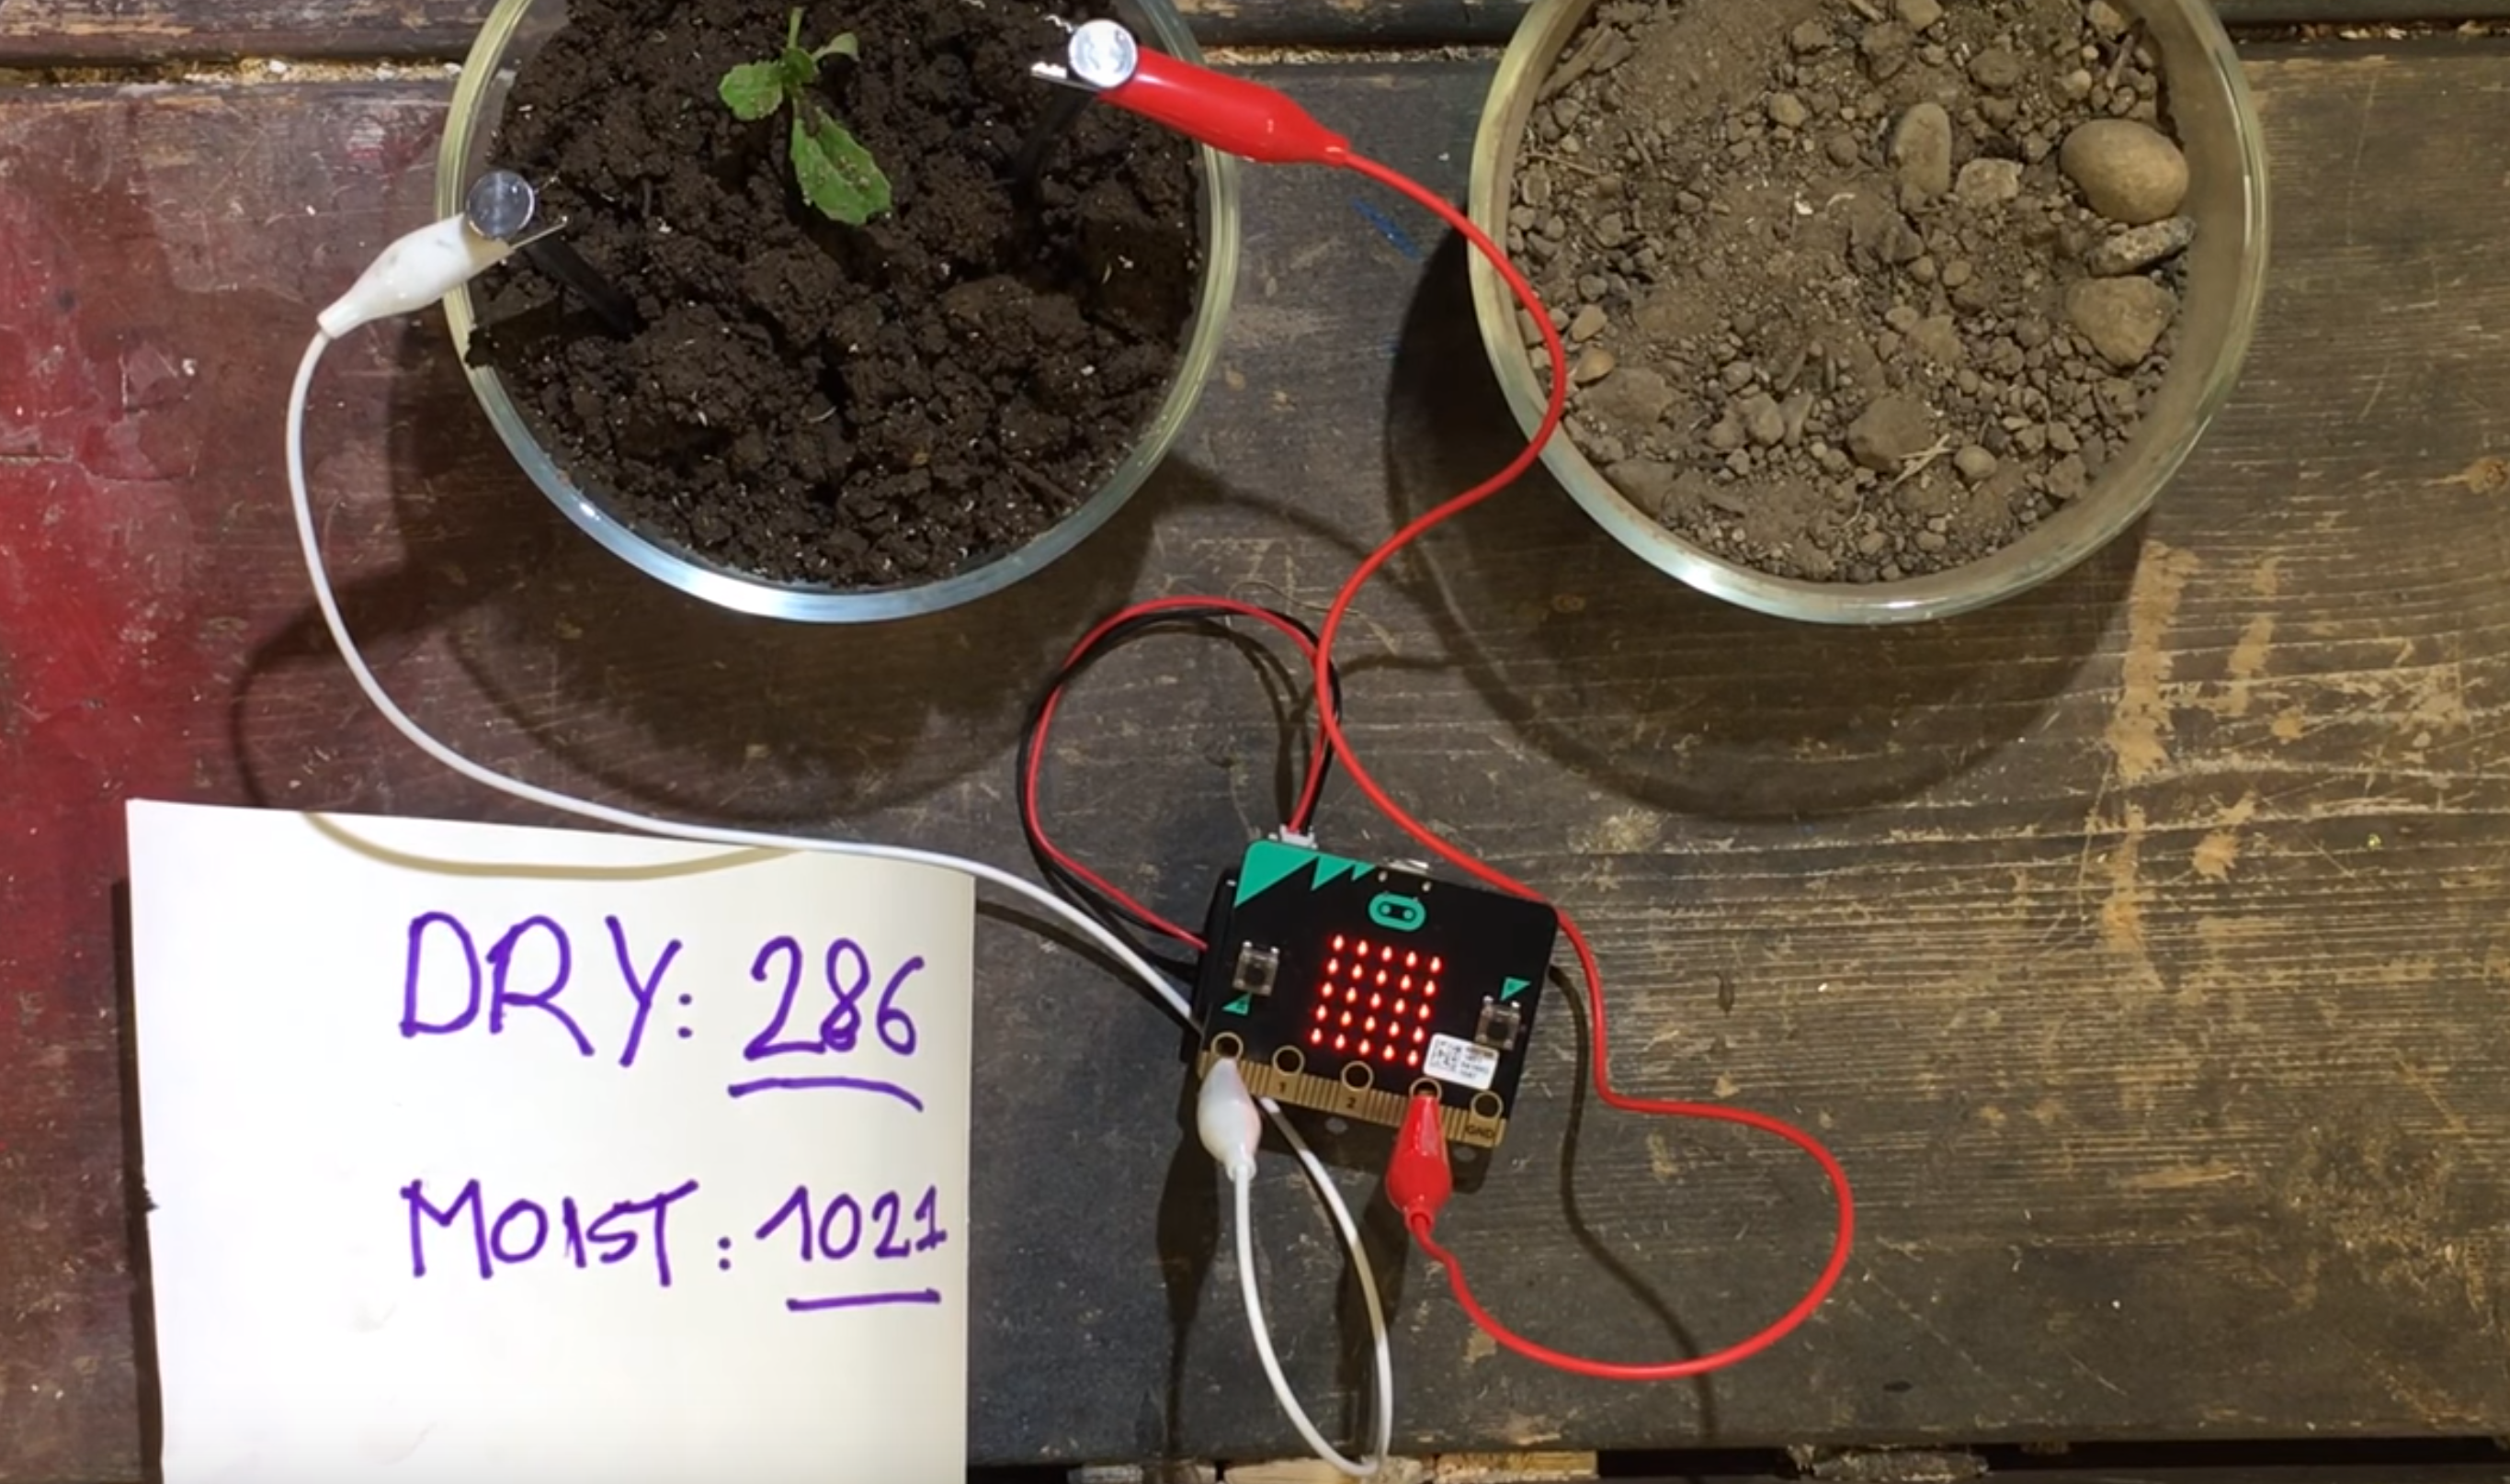
\includegraphics[width=3.3in]{images/moisture.jpg} 
    \includegraphics[width=3.3in]{images/moistureBlocks.png} 
    \caption{\label{fig:moisture}Measuring soil moisture via micro:bit pins.}
\end{figure}

Figure~\ref{fig:moisture} shows an environmental project that uses the 
micro:bit to measure soil moisture. The combination of water 
and soil nutrients makes the soil have some conductivity. The more water there is
in the soil, the greater its conductivity, which can be measured using
the analog pin API. In this project, the student
first learns to calibrate the measurement readings using dry and wet 
soil samples.  Then, the micro:bit is coded to periodically record the
reading. Using the micro:bit's Bluetooth radio, the readings also can
be sent to a central source.  In this way, the moisture of a set of soil
samples (in a classroom) can be recorded and reported. For more about this
project, see:
\begin{center}    
    \small{\url{makecode.microbit.org/projects/soil-moisture}}
\end{center} 

\begin{figure}[t]
\begin{verbatim}
  input.onButtonPressed(Button.A, () => {
    radio.sendString("H");
  });

  input.onButtonPressed(Button.B, () => {
    radio.sendString("S");
  });

  radio.onDataReceived(() => {
    let data = radio.receiveString();
    if (data == "H") {
      basic.showIcon(IconNames.Happy)
    } else if (data == "S") {
      basic.showIcon(IconNames.Sad)
    } else {
      basic.showString("?");
    }
  });
\end{verbatim}
\caption{\label{fig:mood}. Broadcasting simple messages using the micro:bit radio.}
\end{figure}

\subsection{Network}

Using a lower level of the Bluetooth stack, the micro:bit supports 
a simple radio broadcast protocol that can be used to send short messages
to a set of micro:bits. Figure~\ref{fig:mood} presents a simple example 
in JavaScript that shows how to use a micro:bit to communicate your 
``mood'' to other micro:bits in the vicinity.
Note that the micro:bit that sends a message does not
receive that message. 

The following two projects use the micro:bit radio to illustrate
how fireflies synchronize their blinking and how infections spread:
\begin{center}    
    \small{\url{makecode.microbit.org/projects/fireflies}}
\end{center}
\begin{center}    
    \small{\url{makecode.microbit.org/projects/infection}}
\end{center}

\subsection{Control}

The micro:bit can be attached to external actuators, such as servos,
to create systems that respond physically to their environment. 

% light sensor and servo
% https://makecode.microbit.org/projects/milk-carton-robot



% \section{The BBC micro:bit and the Foundation}
% \label{sec:mef}

% In December 2014, the BBC issued an Request for Participation
% for ``Delivery of a hands-on learning experience for the Make it Digital season'',
% which was the micro:bit project.
% Twenty-nine partners were invited to contribute hardware, software, services, 
% teaching materials, packing/distribution, logistics, events and funding.
% Work on the project commenced in February 2015, with delivery of
% a web site/app in September 2015 (which was critical
% for training teachers) and delivery of the micro:bits in the second
% half of the 2015-2016 school year.

% % from: http://microbit.org/about/

% Founded in September 2016,
% the Micro:bit Educational Foundation is a non-profit organization
% legally established with the support of its founding partners~\footnote{ARM,
% Amazon, BBC, British Council, IET, Lancaster University, Microsoft,
% Nominet, and Samsung}. 
% The Foundation's Mission Statement is to: 
% \begin{itemize}
% \item  enable and inspire all children to participate in the digital world, 
% with particular focus on girls and those from disadvantaged groups.
% \item make micro:bit the easiest and most effective learning tool for digital skills and creativity.
% \item work in collaboration with educators to create and curate exceptional 
% curriculum materials, training programmes and resources.
% \item build and support communities of educators and partners 
% to remove the barriers to learning digital skills
% \end{itemize}
% The Foundation works to make micro:bits available for purchase (singly and in bulk)
% around the world through resellers.~\footnote{Currently in 
% Australia, Belgium, Brazil, Canada, China, Croatia, Czech Republic, 
% Denmark, Estonia, Finland, France, Germany, Hong Kong, Hungary, India, 
% Ireland, Israel, Italy, Japan, Latvia, Lithuania, Luxembourg, Malaysia, 
% Netherlands, New Zealand, Norway, Poland, Singapore, Slovak Republic, 
% South Africa, Spain, Sweden, Switzerland, Taiwan, Thailand, UK, and the US.}
% The Foundation redistributes the bulk of any surplus money 
% generated into providing free devices to exceptional 
% micro:bit educational programmes across the globe.

% % country deployments
% \section{Country Deployments}
\label{sec:country}

% rollout
% - UK
%   - http://mb4ps.co.uk/ 
% - Finland
% - Canada: http://microbit.org/en/2018-03-13-cancode-microbit-funding/ 
% - Denmark: http://microbit.org/en/2018-05-07-dr-announcement/ 

% https://github.com/carlosperate/awesome-microbit

localization - language but also curriculum standards

\section{Conclusion}
\label{sec:conclude}

We have presented \MCN: a \emph{no installation}, web-based programming environment, that supports novice programmers with \emph{block-based and text-based higher-level languages}, and compiles programs \emph{in the browser}. So as to not compromise the spatial efficiency of the microcontroller, we created \CON: a C++ runtime that \emph{bridges the semantic gap} between higher level languages in \MC and C++. To transfer programs compiled by \MC to the microcontroller without the installation of any drivers, we created \UFN: a new bootloader and file format that enables the \emph{simplified}, \emph{driverless} programming of microcontrollers.

Combined, our approach to running higher level languages on microcontrollers is up to 50x more performant compared to other approaches. Further, by using modern tooling, and higher level languages, our approach lowers the barrier to entry for microcontroller programming.

% We have presented and evaluated a new platform designed to bring modern language features and tooling to microcontrollers. Our aim was to do this in an extensible way which supports novice programmers with block-based programming while providing a progression path to a text-based scripting language and ultimately to C++. Our platform includes a new C++ runtime called \CO which is designed to make efficient use of the limited resources on a microcontroller. A statically-typed subset of TypeScript forms the basis for both blocks- and text-based programs, created and compiled using a new web-based IDE named \MC.

% Our aspiration is to enable a new paradigm for programming pretty-much anything, even an Arduino Uno-class MCU, by anyone -- novices and professional developers alike, from anywhere, i.e. without the need for traditional heavyweight embedded toolchains and IDEs. Our open-source implementation is in daily use, with thousands of users writing programs targeted at several different MCU-based devices. In this sense, we have achieved our goal. We also have anecdotal evidence that our platform -- in terms of both language and tooling -- is intuitive to professional developers with no experience of embedded development.


%ACKNOWLEDGMENTS are optional
\section{Acknowledgments}

% The following two commands are all you need in the
% initial runs of your .tex file to
% produce the bibliography for the citations in your paper.
\bibliographystyle{abbrv} % standard abbrv style
\bibliography{paper}  % substitute the name of 'your' Bibliography here
% You must have a proper ".bib" file
% and remember to run:
% latex bibtex latex latex (in that particular order) in order to resolve all the 'numerical values'
% be they for figures, equation numbers, references, footnotes, etc. etc.
%
\balancecolumns
% That's all folks! % GM Sept. 2008
\end{document}
